\documentclass[12pt, titlepage]{article}

\usepackage{booktabs}
\usepackage{tabularx}
\usepackage{hyperref}
\usepackage[section]{placeins}
\usepackage{enumitem}
\usepackage{graphicx}
\hypersetup{
    colorlinks,
    citecolor=black,
    filecolor=black,
    linkcolor=red,
    urlcolor=blue
}
\usepackage[round]{natbib}
\newlist{FR}{enumerate}{1}
\setlist[FR]{label=FR\arabic*. }
\title{SE 3XA3: Software Requirements Specification\\BigTwo}

\author{Team 06, Aplus^3
		\\ Jiaxin Tang and tangj63
		\\ Manyi Cheng and chengm33
		\\ Senni Tan and tans28
}

\date{\today}

\begin{document}

\maketitle

\pagenumbering{roman}
\tableofcontents
\listoftables
\listoffigures

\begin{table}[bp]
\caption{\bf Revision History}
\begin{tabularx}{\textwidth}{p{3cm}p{2cm}X}
\toprule {\bf Date} & {\bf Version} & {\bf Notes}\\
\midrule
Feb 9th & 1.0 & Initial Draft\\
Date 2 & 1.1 & Notes\\
\bottomrule
\end{tabularx}
\end{table}

\newpage

\pagenumbering{arabic}

This document describes the requirements for ....  The template for the Software
Requirements Specification (SRS) is a subset of the Volere
template~\citep{RobertsonAndRobertson2012}.  If you make further modifications
to the template, you should explicity state what modifications were made.

\section{Project Drivers}

\subsection{The Purpose of the Project}
The goal of this project is to re-implement the classic LAN party game BigTwo with accurate rules and appropriate documentation.The re-implementation of the Game will be for web browsers such that the player can play BigTwo on their own without finding and gathering other players, and also advance their skills in BigTwo.

\subsection{The Stakeholders}

\subsubsection{The Client}
The clients of this product are the teaching Assistants and Instructor of the course SE 3XA3. They are responsible for supervising the project, they have a basic understanding of the project and keep track of the project progress through various milestones, and they will be actively involved in the development process of the project.

\subsubsection{The Customers}
The customers for the product are the general public of any ages with knowledge and physical ability to read and understand English, and basic operation of a computer and web browser, who are interested in the BigTwo card game. Customers of this product are also those users who are interested in advancing their skills in this game.

\subsubsection{Other Stakeholders}
\begin{itemize}
    \item General Public and Users - These are the main users intended to use the product after release. They require little or no understanding of the project but should be able to use the product.
    \item Group 6 - As the developers of the game, we hold responsibilities to ensure that this game successfully meets the requirements and goals that are outlined. All members should be involved in various software development phases of this project.
\end{itemize}

\subsection{Mandated Constraints}
\subsubsection{Product Constraints}
In order to use the product, an internet connection and a web browser are required for the user. Mainstream Web browsers that support JS ES6 and HTML5 are required to run the web application. Users also need to remain connected to the internet throughout the entire game after the web page is loaded.
\subsubsection{User Constraints}
Users and players of the product must have knowledge and physical ability to read and understand English, and basic operation of a computer with mouse/pad and web browser.
\subsubsection{Time Constraints}
The deadline of this project is April 12, 2021. All the development and documentation of this project should be delivered by the deadline, and this limits the amount of features and compromises product quality on the initial release of the software.
\subsubsection{Budget Constraints}
There is no budget for this project so all the software and resources used in this project must be free, and this may limits the amount of features and the quality of user experience.
\subsection{Naming Conventions and Terminology}
\begin{itemize}
    \item Python - An interpreted, high-level and general-purpose programming language. 
    \item JavaScript - A programming language that conforms to the ECMAScript specification.
    \item HTML - Hypertext Markup Language (HTML) is the standard markup language for documents designed to be displayed in a web browser. 
    \item CSS - Cascading Style Sheets (CSS) is a style sheet language used for describing the presentation of a document written in a markup language.
    \item PyGame - A cross-platform set of Python modules designed for writing video games. It includes computer graphics and sound libraries designed to be used with the Python programming language. 
    \item Open source - Open source is source code that is made freely available for possible modification and redistribution.
    \item User interface - The space where interactions between humans and machines occur.
\end{itemize}

\subsection{Relevant Facts and Assumptions}
We assume that the users and players of the product have the knowledge and physical ability to read and understand English, and basic operation of a computer with mouse and web browser so no extra instruction or resources of these will be provided during the game.

\section{Functional Requirements}

\subsection{The Scope of the Work and the Product}
The software product for this project is a BigTwo game on major web browsers. The BigTwo game will emulate playing the game of bigtwo with 3 computer bots using standard rules. The BigWwo game being implemented will not have multiplayer functionality and no other game functionality beyond BigTwo.
The goal of this software system is to allow beginners learn about BigTwo, as well as providing a portable platform for players to play BigTwo on their own in this pandemic situation. The objective that this software system aims to achieve is to provide users
with an entertaining and visually pleasing environment to play the game of
BigTwo. The benefits that this software system provides to users is that by playing
BigTwo in an emulation environment without real money, users can practice BigTwo and learn rules faster.

\bigskip
\newline

\noindent \subsubsection{Deadlines and Deliverables}
\begin{itemize}
\item Project Approval -- January 25
\item Problem Statement -- January 29
\item Development Plan -- Feb 5
\item Requirements Document Revision 0 -- February 12
\item Proof of Concept Demonstration -- Week of February 22 
\item Test Plan Revision 0 -- March 5
\item Design & Document Revision 0 -- March 18
\item Revision 0 Demonstration -- Week of March 22
\item Final Demonstration (Revision 1) -- Week of Apr 5
\item Final Documentation (Revision 1) -- April 12
    \begin{itemize}
        \item Problem Statement
        \item Development Plan
        \item Requirements Document
        \item Design Document
        \item Test Plan
        \item Test Report
        \item Source Code
    \end{itemize}
\end{itemize}

\FloatBarrier
\subsubsection{The Context of the Work}
\bigskip
\begin{figure}[h!]
    \centering
    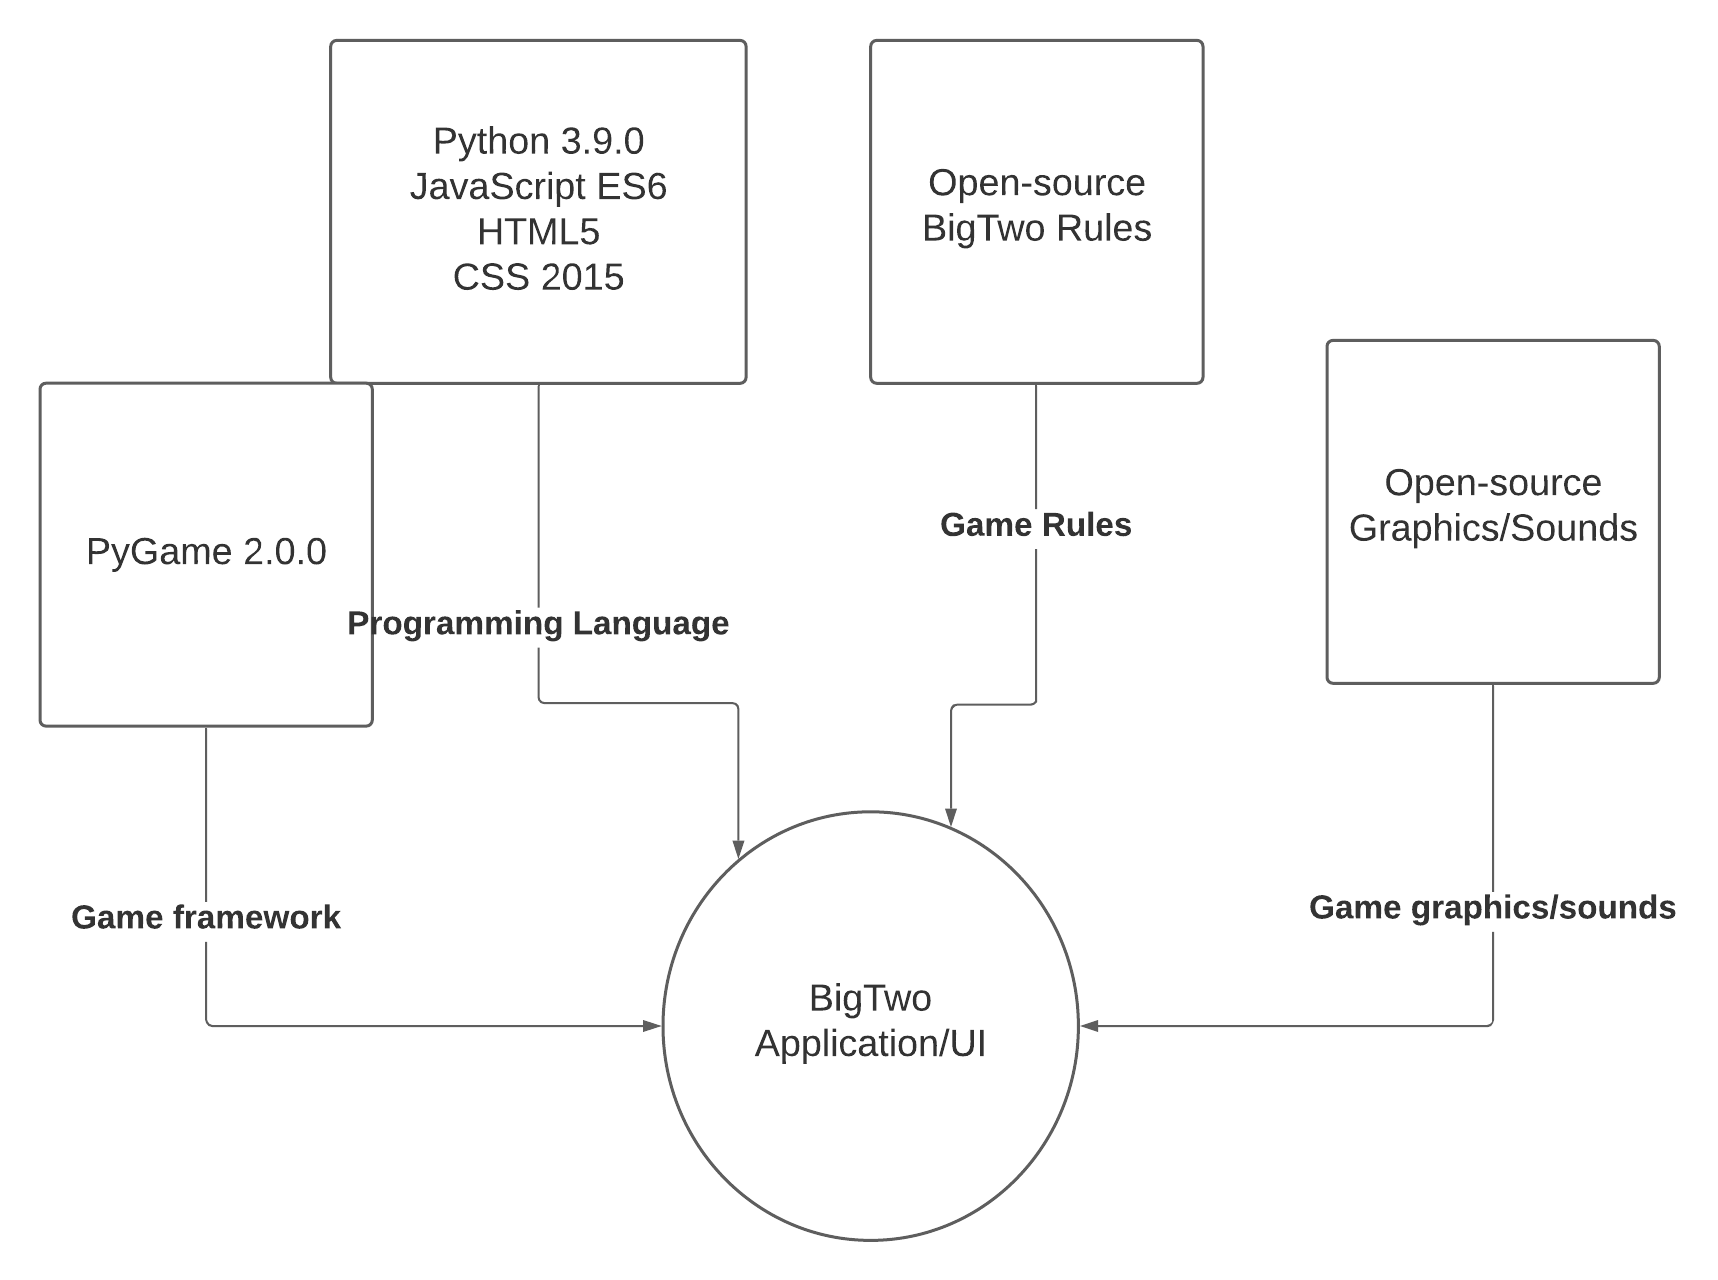
\includegraphics[width=0.9\textwidth]{context_of_work.png}
    \caption{Context the the Work for BigTwo}
    \label{fig: context of work}
\end{figure}

\FloatBarrier
\subsubsection{Work Partitioning}
\newpage
\begin{table}[h!]
\begin{center}
\begin{tabularx}{\textwidth}{ |X|X|X| } 
\hline
Event Name & Input  & Summary\\ 
\hline
1.Gather rules for standard BigTwo game & Wikipedia & Rules for Standard BigTwo are found on Wikipedia and
available to be followed for our implementation of BigTwo\\
\hline
2.Player perform action & HTTP Request & Process player's request and modify game state\\
\hline
3.Computer bot perform action & HTTP Request & Calculate the best move using AI and modify the game state\\
\hline
\end{tabularx}
\end{center}
\caption{Work Partitioning}
\label{table:1}
\end{table}
\subsubsection{Individual Product Use Cases}
\begin{itemize}
    \item  A user plays a game of Standard BigTwo.
    \item A user starts a round.
    \item The first dealer is picked randomly.
    \item The user wants to deal out cards singly.
    \item The user wants to deal out cards as part of combination.
    \item The user wants to pass.
    \item The user wants to pause.
    \item The user wants to play again.
    \item The user wants to exit the game.
    
\end{itemize}
\FloatBarrier
\subsection{Functional Requirements}
\begin{FR}
\item The user must be able to play a game of BigTwo.\\
Fit Criterion: The user is able to select the appropriate game mode by clicking the navigation.
\item The user interface must notify the user the results of a round.\\
Fit Criterion: The user interface will display an alert message to the screen
\item The user interface must notify the user the results of a round.\\
Fit Criterion: The user interface will display an alert message to
inform the user if they have won or lost, and the score of the player
and dealer is indicated on the screen scoreboard for the round.
\item The game interface must display the interactive deck of cards the user possesses. \\
Fit Criterion: The game interface must display the deck of cards the user possesses such that each card can be selected by the user upon clicking it.
\item The user interface must include an image to represent the background
of the game.\\
Fit Criterion: The BigTwo table image with a background color to
represent the theme of the game will be presented in the user interface.
\item The user interface must include a button for the user to indicate their action to deal.\\
Fit Criterion: The deal Button will appear once the user selects certain cards from their set when it is user's turn after entering the game by clicking the play game button.
\item The user interface must include a button for the user to indicate their action to pass.\\
Fit Criterion: The pass Button will appear once the game proceeds to user's turn after entering the game by clicking the play game button.
\item The user interface must display how many cards each other player possesses without revealing actual card sets.\\
Fit Criterion: Back of card set will be shown on the screen once the user clicks on the play game button.
\item The user interface must indicate who is the current dealer.\\
Fit Criterion: Current dealer will be shown by each player's icon once the user clicks on the play game button.
\item The user interface must include a button for the user to indicate their action to pause.\\
Fit Criterion: The pause button will appear in upper right corner of the game.
\item The user interface must include a button for the user to indicate their action to exit.\\
Fit Criterion: The exit button will appear in upper right corner of the game right beside pause button.
\item The user will start the game with STARTING DECK OF CARDS.\\
Fit Criterion: The user will start the game with a random deck of cards.

\end{FR}

\FloatBarrier
\section{Non-functional Requirements}

\subsection{Look and Feel Requirements}
\subsubsection{Appearance Requirements}
\begin{enumerate}
    \item The product shall display the name of the product and the logo of the company upon starting.
    \item The product shall have clearly labelled buttons.
    \item The product shall have a proper size to fit on a web page.
    \item The product shall appear attractive to users.
\end{enumerate}

\subsubsection{Style Requirements}
\begin{enumerate}
    \item The product shall generate cards in a clear way.
    \item The color of the cards shall be distinct from the background. 
\end{enumerate}
\subsection{Usability and Humanity Requirements}
\subsubsection{Ease of Use requirements}
\begin{enumerate}
    \item The product shall only require the users' mouse for navigating the menu and selecting cards to play the game.
    \item The product shall be easy for users with rules of the game provided.
\end{enumerate}

\subsubsection{Personalization and Internationalization Requirements}
\begin{enumerate}
    \item The product shall be provided in English.
\end{enumerate}

\subsubsection{Learning Requirements}
\begin{enumerate}
    \item The user shall be able to operate a mouse and a web browser.
    \item The product shall provide a simple instruction of the game for users.
\end{enumerate}

\subsubsection{Understandability and Politeness Requirements}
\begin{enumerate}
    \item The product shall use an average level of vocabulary.
    \item The product shall be easy for users age 14 and above.
\end{enumerate}

\subsection{Accessibility Requirements}
\begin{enumerate}
    \item The product shall be executable on the majority of computers and web browsers.
\end{enumerate}

\subsection{Performance Requirements}
\subsubsection{Speed and Latency Requirements}
\begin{enumerate}
    \item The product shall respond to each user input within 2 seconds.
\end{enumerate}

\subsubsection{Safety-Critical Requirements}
\begin{enumerate}
    \item The product shall not compromise the user data or computers.
\end{enumerate}

\subsubsection{Precision or Accuracy Requirements}
\begin{enumerate}
    \item The product shall respond to each user input correctly according to the rules of BigTwo game.
\end{enumerate}

\subsubsection{Reliability and Availability Requirements}
\begin{enumerate}
    \item The product shall be available at any time when users have access to a web browser.
    \item The product shall never crash.
\end{enumerate}

\subsubsection{Robustness or Fault-Tolerance Requirements}
\begin{enumerate}
    \item The product shall not give output if a users gives an undesired input.
\end{enumerate}

\subsubsection{Capacity Requirements}
\begin{enumerate}
    \item The product shall not exceed the server load.
\end{enumerate}

\subsubsection{Scalability or Extensibility Requirements}
N/A

\subsubsection{Longevity Requirements}
\begin{enumerate}
    \item The product shall always be functional with a relevant web browser.
\end{enumerate}

\subsection{Operational and Environmental Requirements}

\subsubsection{Expected Physical Environment}
\begin{enumerate}
    \item The product shall be available for any device that has access to a web browser.
\end{enumerate}

\subsubsection{Requirements for Interfacing with Adjacent Systems}
\begin{enumerate}
    \item The product shall be available for any device that has access to a web browser. 
\end{enumerate}

\subsubsection{Installability Requirements}
N/A

\subsubsection{Release Requirements}
\begin{enumerate}
    \item The new release of the product shall not cause the previous version to fail.
    \item The product shall be updated if there are some errors or bugs upon realization.
\end{enumerate}

\subsection{Maintainability and Support Requirements}
\subsubsection{Maintenance Requirements}
\begin{enumerate}
    \item The product shall undergo revision yearly.
\end{enumerate}

\subsubsection{Supportability Requirements}
\begin{enumerate}
    \item The product shall be available for the majority of the web browsers.
\end{enumerate}

\subsubsection{Adaptability Requirements}
\begin{enumerate}
    \item The product shall be compatible with the majority of the web browsers.
\end{enumerate}

\subsection{Security Requirements}
\subsubsection{Access Requirements}
\begin{enumerate}
    \item The source code of the product shall be only authorized for developers.
\end{enumerate}

\subsubsection{Integrity Requirements}
\begin{enumerate}
    \item The product shall not accept incorrect user data or user input.
\end{enumerate}

\subsubsection{Privacy Requirements}
\begin{enumerate}
    \item The product shall not require any personal information from users.
\end{enumerate}

\subsubsection{Audit Requirements}
\begin{enumerate}
    \item The product shall be audited yearly.
\end{enumerate}

\subsubsection{Immunity Requirements}
N/A

\subsection{Cultural Requirements}
\begin{enumerate}
    \item The product shall not use any words or graphics that are offensive to people with any culture.
\end{enumerate}

\subsection{Legal Requirements}
\subsubsection{Compliance Requirements}
\begin{enumerate}
    \item The product shall not violate any laws.
\end{enumerate}

\subsubsection{Standards Requirements}
\begin{enumerate}
    \item The product shall follow the MIT Open License.
\end{enumerate}

\subsection{Health and Safety Requirements}
\begin{enumerate}
    \item The product shall prevent users from game addiction.
    \item The product shall not involve any gambling elements.
\end{enumerate}


\section{Project Issues}

\subsection{Open Issues}
Understanding of code structure of existing open-source project found on GitHub.
\begin{itemize}
    \item The original project on GitHub was implemented in Java. We will analyze and re-implement the modules in Python.
\end{itemize}
\subsection{Off-the-Shelf Solutions}
\subsubsection{Existing Products}
There are many existing products for that have created the game of BigTwo. They are listed below:
\begin{itemize}
    \item Play Big Two Cards Game Online (http://www.onlinesologames.com/bigtwo)
    \item Big 2 - Card Game - GamsSlush (https://www.gameslush.com/big-2)
    \item Play Big2 online - PlayDOSGame.com (https://www.playdosgames.com/online/big2/)
\end{itemize}
There are many other variations of BigTwo Game found online. We are going to investigate these ready-made products, find the advantages and drawbacks in their designs, and then improve our design and implementation.
\subsubsection{Ready Made Components}
\begin{itemize}
    \item PyGame
\end{itemize}
\subsubsection{Reusable Components}
N/A
\subsubsection{Products That Can Be Copied}
As an open source project the original implementation can be relied upon as a reference.
\subsection{New Problems}
\subsubsection{Problems in Current Environment}
The new game will be running on a website. If the server hosting the website is crashed, then the the game can not run on the website.
\subsubsection{Effects on the Installed Systems}
This interface stand alone on and does not coexist with an older system.
\subsubsection{Existing Users}
Some potential user problems as an adverse reaction from playing our project are eye soreness and eye strain from extended playing.
\subsubsection{Limitations in implementation environment}
N/A
\subsubsection{Follow Up Problems}
If we one of the developers leave the team, there will be a gap in the information of how the product is implemented. There are also adverse risks if the software becomes too outdated for new upcoming web browsers and technology.

\subsection{Tasks}
\begin{figure}[h]
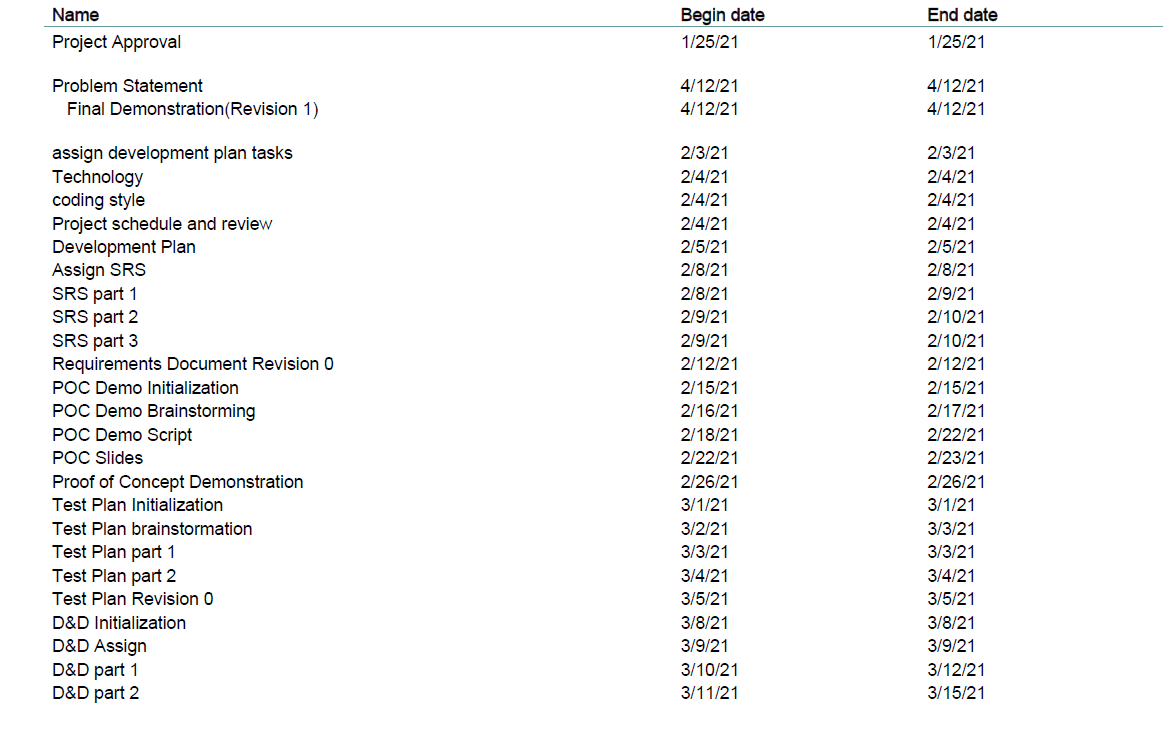
\includegraphics[width=12cm]{task1.png}
\caption{Tasks generated by GanttProject}
\end{figure}
\begin{figure}[h]
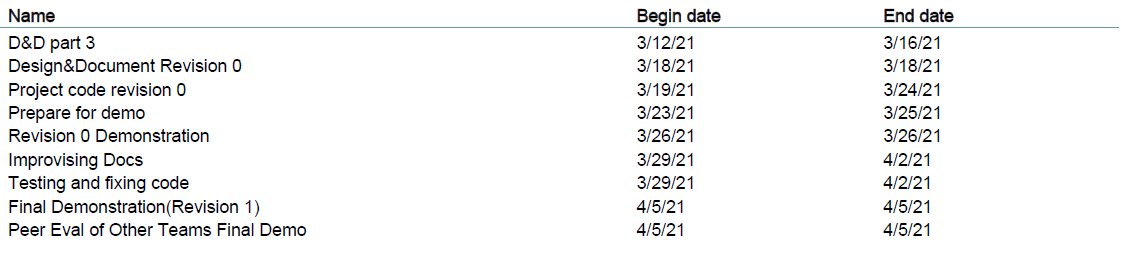
\includegraphics[width=13cm]{task2.png}
\caption{Tasks continue}
\end{figure}

\subsection{Migration to the New Product}
\subsubsection{Requirements for Migration to the New Product}
N/A.
\subsubsection{Data That Has to Be Modified or Translated for the New System}
N/A
\subsection{Risks}
Testing is a risk that must be assessed. The integration testing of the game may be difficult to automate because the program is a game. It requires testing that relies heavily on user testing which is not efficient.
\subsection{Costs}
None as long as the software and other resources used in this project is free.
\subsection{User Documentation and Training}
\subsubsection{User Documentation Requirements}
N/A
\subsubsection{Training Requirements}
N/A

\subsection{Waiting Room}
Additional functionality of the game and visual as well as audio effects.

\subsection{Ideas for Solutions}
Proper hierarchy and documentation of Python code for the game and JavaScript, HTML, CSS code for the web interface.

\section{Appendix}
N/A
%This section has been added to the Volere template.  This is where you can place
%additional information.

\subsection{Symbolic Parameters}
N/A
%The definition of the requirements will likely call for SYMBOLIC\_CONSTANTS.
%Their values are defined in this section for easy maintenance.

\newpage
\bibliographystyle{plainnat}

\bibliography{SRS}


\end{document}